As a new idea, this study introduces the concept of trustless transport which replaces the need of centralized intermediation of supply and demand. We propose a mechanism which punishes hostile actors automatically resulting in no conflict resolution required from central entities. The meaning of used abbreviations in this chapter can be found in the list of symbols appendix A.\par
In our scenario seen at figure \ref{fig:1 main overview}, we assume that the service consumer $A$ wants to send an physical asset to the endpoint actor $B$. The third and last actor is the service provider $C$ who will execute the transport contract. Let $A$, $B$ and $C$ all have an ECDSA key pair and Bitcoin address. \[GenerateAddress(PubK_n)\colon Adr_n\]
The scenario starts of with $A$ creating a Ricardian contract representing a request for transport, this contract minimally contains $B$ public key, $B$ location, $A$ location, physical asset equivalent cost and the transport reward.
\[Rc \supseteq \{PubK_b, Loc_b, Loc_a, EqC, Tr\}\]
This contract is accepted by $C$ which then signs an unspent transaction from $Adr_c$, denoted by $tx_1$, containing the physical asset equivalent cost or more to the $2/2$ multisignature address of the service provider and endpoint actor
\[SignTransaction(PrivK_c)\colon\{EqC, Adr_C, MSig_{bc}\}\mapsto tx1\].

\begin{figure}[h]
\centering
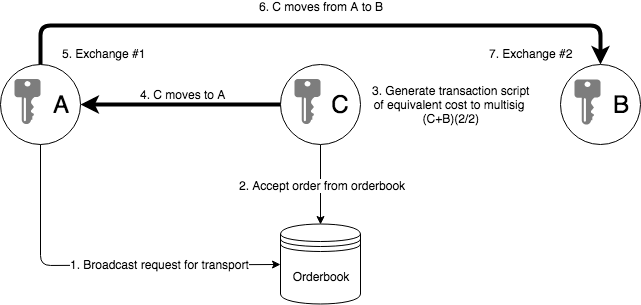
\includegraphics[width=1\textwidth]{images/main.png}
\caption{Overview test scenario}
\label{fig:1 main overview}
\end{figure}

Upon accepting $C$ moves to the physical location of $A$ bringing transaction script $tx_1$. As illustrated with figure \ref{fig:2 first exchange}, upon $C$ arriving at $A$ the asset pickup exchange can take place.

\begin{enumerate}
  \item $C$ innitiates the exchange by giving $A$ the transaction script $tx_1$
  \item $A$ signs a unspent transaction from $Adr_a$ to the multisignature address containing the reward for transporting the physical asset. \[SignTransaction(PrivK_a)\colon\{Tr, Adr_a, MSig_{bc}\}\mapsto tx_2\]
  \item $A$ broadcasts the transport incentive into escrow $\{tx_1, tx_2\}$
  \item $A$ signs and broadcasts the ownership change of the $Rc$ from $A\rightarrow C$
  \item Wait block confirmation containing $\{tx_1, tx_2\}$
  \item Exchange the physical asset from $A\rightarrow C$
\end{enumerate}

Before $\{tx_1, tx_2\}$ get broadcasted \textit{A $\lor$ C} can individually verify if the signed transactions actually contain what they should.

\begin{figure}[h]
\centering
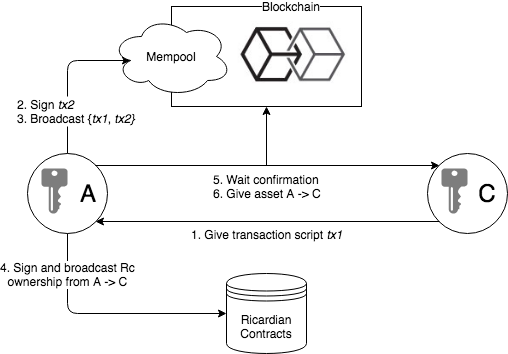
\includegraphics[width=0.8\textwidth]{images/exchange_01.png}
\caption{Asset Pickup Exchange}
\label{fig:2 first exchange}
\end{figure}

 When \textit{C} recieves the physical asset he is the custodian and will move to the endpoint $Loc_b$ to claim the reward locked in the escrow. As illustarted with figure \ref{fig:3 dropoff exchange}, upon \textit{C} arriving at $Loc_b$ the physical asset dropoff exchange takes place which consist out of the following steps:

\begin{enumerate}
  \item $B$ signs $tx_3$ containing the equivalent value and transporting reward from $MSig_{bc}$ to $Adr_c$
  \[SignTransaction(PrivK_b)\colon\{\{tx_1, tx_2\}, MSig_{bc}, Adr_c\}\mapsto tx_3\]
  \item $B$ gives the transaction script $tx_3$ to $C$
  \item $C$ signs and broadcasts the ownership change of the $Rc$ from $C\rightarrow B$
  \item Exchange physical asset from $C\rightarrow B$
\end{enumerate}

\begin{figure}[h]
\centering
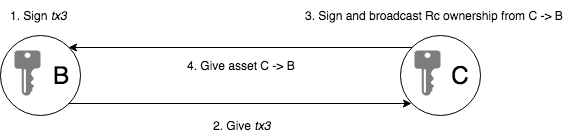
\includegraphics[width=0.8\textwidth]{images/exchange_02.png}
\caption{Asset Dropoff Exchange}
\label{fig:3 dropoff exchange}
\end{figure}

At the end of the second exchange actor $C$ now owns $tx_3$ which has been signed by $B$. He can now sign and broadcast the transaction with his own keypair whenever he wants to redeem the funds.

\[SignTransaction(PrivK_c)\colon\{\{tx_1, tx_2\}, MSig_{bc}, Adr_c\}\mapsto tx_3\]
